  \def\firstcircle{(0,0) circle (1cm)}
  \def\secondcircle{(1,0) circle (2cm)}
  \centering
  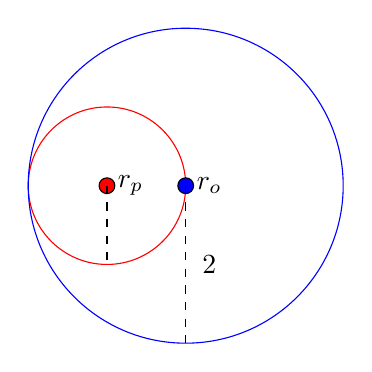
\begin{tikzpicture}
    % \begin{scope}
    %     \clip \firstcircle;
    %     \fill[filled] \secondcircle;
    % \end{scope}
    \draw[color=red]  \firstcircle;
    \draw[color=blue] \secondcircle;

    \draw[fill=red] (0, 0) circle (0.1cm); 
    \node at (0.3, 0) {$r_p$};
    \draw[fill=blue] (1, 0) circle (0.1cm); 
    \node at (1.3,0) {$r_o$};
    \draw[dashed](0, 0) -- (0,-1);
    \node at (-0.3, -0.5) {$\range$};
    \draw[dashed](1, 0) -- (1,-2);
    \node at (1.3, -1) {$2\range$};
  \end{tikzpicture}
  \caption{}